\subsection{State space controller}

In chapter \ref{chapter_StateSpace} the basic idea of the state space representation is explained. This chapter deals with the part, controlling the process of \myfigref{fig:simpleProcess}. 

But how to do that?

One possibility is, to use several PI(D) controllers in an cascade control architecture, but - in this case - a state space controller is the candidate. The fundamental idea of this controller is, to feed back all required internal state variables. In the feedback of each state variable, there has to be a specific factor. The method used in this project to determine these factors, is the pole placement (chapter \ref{chapter_PolePlace}). In order to be able to develop a state space controller for a process - as the dynamics of the quadrocopter - it is necessary, that the process is controllable.

How does a state space controller for the process of \myfigref{fig:simpleProcess} look like?

\begin{figure}
	\centering
		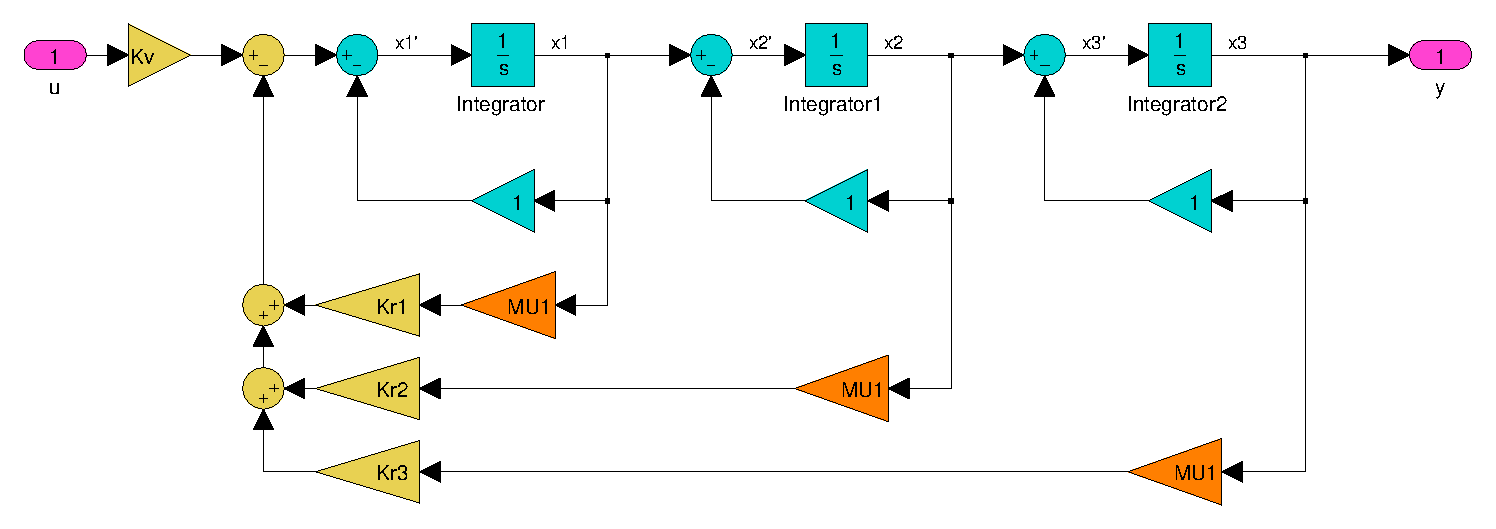
\includegraphics[width=1.00\textwidth]{03_Grafiken/simpleProcess_Controller.pdf}
	\caption{Simple process example including the state space controller}
	\label{fig:simpleProcess_Controller}
\end{figure}

There it is - the controller for the simple process of \myfigref{fig:simpleProcess}. The orange marked \textit{MUx} are the measuring converters, that are not important in this simple example. That is, why they are not described more precisely in this chapter. 
The controller is the whole part, marked in yellowish brown. On the one hand there are the feedback factors \textit{KRx}, on the other hand there is the pre-intensification factor \textit{Kv}. All in all, there are four independent parameters, which have to be calculated while designing the state space controller. For a MIMO system, chapter \ref{chapter_MIMO} deals with, there are much more independent parameters that have to be defined while designing.
As mentioned, the pre-intensification factor \textit{Kv} is one part of the controller. Its function is, to reduce the steady control deviation. How this factor and the other part of the state space controller, the feedback factors \textit{KRx}, are calculated, is described in the chapter \ref{chapter_PolePlace} pole placement.

